\section{Motivating Example}
\label{sec:example}

\begin{lstlisting}[float, label=lst:example, caption={A faulty guard removal from our corpus (\code{Refactorings.ratio}). The edit deletes line 3.}]
static int ratio(int a, int b) {         static int ratio_edited(int a, int b) {
  int d = b - a;                           int d = b - a;
  if (d == 0) return 0;
  return d / (a > b ? a : b);              return d / (a > b ? a : b);
}                                        }
\end{lstlisting}

\Cref{lst:example} shows the original $A$ (left) and the edited version $B$ (right). Both
take two \code{int}s, and we check them on the domain $D = [-3,3]^2$ (49 inputs). The
original also throws on some inputs: for $(0,-1)$ the larger argument is $0$ and
$d = -1 \neq 0$, so both versions divide by zero and \emph{agree}. They disagree on exactly
one input, $(0,0)$, where $A$ returns $0$ and $B$ throws.

\paragraph{What the existing analyses report}
For both versions on $D$, an outcome analysis in the \jpamb{} style gives the outcome set
$\set{\ok, \dbz}$, and so does a perfectly precise one. Comparing outcome sets therefore suggests the edit is
safe. A single SMT query over $D$ that encodes both outcome and return value does find
$(0,0)$, but it stops there: it certifies one input of 49 (2\%), and the developer learns
nothing about the rest. Differential testing with 1000 random inputs finds $(0,0)$ on $D$
after 78 runs, but on $[-1000,1000]^2$ it misses it and can only answer \unk{}.

\paragraph{What our checker reports}
\Cref{fig:ratio} shows the regions our checker produces. The constants in the code are
$\set{0}$, so the first split cuts $a$ into $[-3,-1]$, $[0,0]$ and $[1,3]$, and the next
splits cut $b$ in the boxes with $a \le 0$. Each resulting box is then decided:
\begin{itemize}
  \item On $a \in [0,0], b \in [0,0]$ the interval analysis gives $\set{\ok}$ for $A$
        (refining $d = 0$ selects the guard) and $\set{\dbz}$ for $B$ (the divisor is the
        interval $[0,0]$). The sets are disjoint, so the box is \chg{} on \emph{every}
        input and $(0,0)$ is a witness (Rule~2 in \cref{sec:formal}).
  \item On $a \in [-3,-1], b \in [0,0]$ and on $a \in [0,0], b \in [-3,-1]$ the larger
        argument is $0$ and $d \neq 0$, so both versions have outcome set
        $\set{\dbz}$: the box is \pres{} without looking at values (Rule~1).
  \item The four remaining boxes have outcome set $\set{\ok}$ for both versions, but the
        return intervals overlap. Here, and only here, the checker asks Z3 whether some
        input in the box makes the return values differ. All four queries are UNSAT, so the
        boxes are \pres{} (Rule~3).
\end{itemize}
The verdict is \chg{} with witness $(0,0)$ and a certified coverage of 100\%: 48 inputs
are proved \pres{} and one is proved \chg{}. This took 10 region analyses and 4 SMT
queries. On $[-1000,1000]^2$ the same 10 regions and 4 queries arise,
and coverage again reaches 100\%.

\begin{figure}
  \centering
  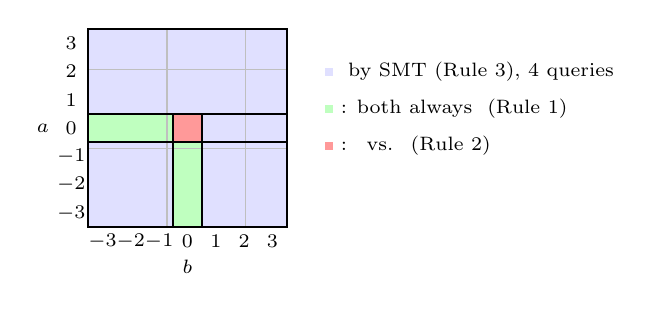
\begin{tikzpicture}[x=0.36cm, y=0.36cm, font=\scriptsize]
    \def\cell#1#2#3{\fill[#3] (#1,#2) rectangle ++(1,1);}
    % b on x-axis (-3..3 -> 0..6), a on y-axis (-3..3 -> 0..6)
    \fill[blue!12] (0,0) rectangle (3,3);   % a<0, b<0: SMT
    \fill[blue!12] (4,0) rectangle (7,3);   % a<0, b>0: SMT
    \fill[green!25] (3,0) rectangle (4,3);  % a<0, b=0: rule 1
    \fill[green!25] (0,3) rectangle (3,4);  % a=0, b<0: rule 1
    \fill[red!40]   (3,3) rectangle (4,4);  % (0,0): rule 2
    \fill[blue!12] (4,3) rectangle (7,4);   % a=0, b>0: SMT
    \fill[blue!12] (0,4) rectangle (7,7);   % a>0: SMT
    \draw[gray!50] (0,0) grid (7,7);
    \draw[thick] (0,0) rectangle (7,7);
    \draw[thick] (0,4) -- (7,4) (0,3) -- (7,3);
    \draw[thick] (3,0) -- (3,4) (4,0) -- (4,4);
    \foreach \v [count=\i from 0] in {-3,...,3} {
      \node at (\i+0.5,-0.5) {$\v$};
      \node at (-0.6,\i+0.5) {$\v$};
    }
    \node at (3.5,-1.4) {$b$};
    \node at (-1.6,3.5) {$a$};
    \node[anchor=west, align=left] at (8,5.5) {\tikz\fill[blue!12] (0,0) rectangle (0.3,0.3); \pres{} by SMT (Rule 3), 4 queries};
    \node[anchor=west, align=left] at (8,4.2) {\tikz\fill[green!25] (0,0) rectangle (0.3,0.3); \pres{}: both always \dbz{} (Rule 1)};
    \node[anchor=west, align=left] at (8,2.9) {\tikz\fill[red!40] (0,0) rectangle (0.3,0.3); \chg{}: \ok{} vs.\ \dbz{} (Rule 2)};
  \end{tikzpicture}
  \caption{Regions decided by the hybrid checker for \code{ratio} on $[-3,3]^2$. Thick lines
  are region borders; every input lies in a region with a proved verdict.}
  \label{fig:ratio}
\end{figure}

\paragraph{A value-only change}
The second kind of edit our approach targets is one where both versions always finish
normally. The corpus pair \code{sign} computes the sign of \code{x} with
\code{if (x > 0) return 1; if (x < 0) return -1; return 0;}. The edit deletes the second
test, so the method ends in \code{return -1}, and at $x = 0$ it returns $-1$ instead of
$0$. Both versions have outcome set $\set{\ok}$ and return interval $[-1,1]$ on every
domain, so no outcome-based analysis can see the change: the difference lies in the
\emph{relation} between input and output. On the whole domain the return query finds the
witness $x = 0$, which replays (Rule~3$'$). That proves the change but certifies one input,
so the checker keeps splitting at the constants of the code. On the point region
$x \in [0,0]$ the return intervals are $[0,0]$ and $[-1,-1]$, which are disjoint, so that
region is \chg{} (Rule~2b). On the regions below and above $0$ both versions return the
same constant, $-1$ or $1$, so those regions are \pres{} (Rule~2b$'$). One input is
\chg{}, the other six are \pres{}, and coverage is 100\%. Even without the solver the
splitting alone reaches the same map.
